%	----- PACKAGES AND OPTIONS ----- 
\documentclass[11pt,a4paper,english,oneside]{article}
\usepackage{etex} %Because of many packages --> Extended TeX.
\usepackage[left=1in, right=1in]{geometry} %Helps to structure the paper layout.
\usepackage[Lenny]{./style/fncychap} %Design of the thesis.
\usepackage[utf8]{inputenc} %Due to vowels.
\usepackage[british]{babel} %Define the language style.
\usepackage{dsfont} %Nice style for the indicator function.
\usepackage{fancyhdr} %To customize the headers and footers.
\usepackage{booktabs} %In case you need \cmidrule or \addlinespace in tables.
\usepackage[hang,bottom,stable,multiple]{footmisc} %Style of footnotes.
%\usepackage{appendix} %For the \appendixpage command.
\usepackage[titletoc,toc,page]{appendix}
%Load some mathematical packages.
\usepackage{amsmath}
\usepackage{amsfonts}
\usepackage{amsmath}
\usepackage{amssymb}
\usepackage{mathtools}
\usepackage[sort,round]{natbib} %For the bibliography.
\usepackage{etoolbox} %To remove the page number on \appendixpage.
\usepackage{amsthm} %For theorems, definitions etc.
\usepackage{thmtools} %For theorems, definitions etc.
\usepackage{setspace} %Use double spacing.
\usepackage{lipsum} %For the \lipsum command to generate a text.
\usepackage{datetime} %For the specification of the date.
%\usepackage{tocloft} %The ToC, LoF and LoT each appear not necessarily on a new page.
\usepackage{graphicx,listings,xcolor,textcomp} %For the graphics, listings etc.
% \usepackage[justification=raggedright,singlelinecheck=true,
%              font=small, labelfont=bf]{caption} %Customize the captions.
\usepackage{caption,threeparttable}
\captionsetup{labelfont=bf,
              justification=raggedright,
              singlelinecheck=false,
              labelfont=bf,
              font=small}
% \usepackage[justification=raggedright,
%             singlelinecheck=false,format=plain]{subcaption}
\usepackage{chngcntr} %To use counterwithout.
\usepackage{epstopdf} %For inserting .eps files into the document.
\usepackage{xparse} %Load for \NewDocumentCommand command.
\usepackage{rotating} %To rotate a table.
\usepackage{pdfpages}
\usepackage{array,hhline} %To create tables and matrices.
\usepackage{tabularx} %An extended version of tabular.
% \usepackage{arydshln} %Due to the capability to draw horizontal/vertical dash-lines.
\usepackage{hyperref} %Must be loaded at the end.
\usepackage{cleveref} %For the command \cref, load after hyperref.
\usepackage{makecell}
\usepackage{cellspace}
\setlength\cellspacetoplimit{4pt}
\setlength\cellspacebottomlimit{4pt}

\graphicspath{ {./../resources/figures/} } %  Figures directory

\renewcommand{\appendixpagename}{\appendixname}
\renewcommand{\appendixtocname}{\appendixname}

\noappendicestocpagenum

%Setup of the reference links.
\hypersetup{
     colorlinks=false,
     linkcolor=blue,
     citecolor=blue,
     filecolor=magenta,
     urlcolor=blue}

%Define some reasonable margins.
\setlength{\textwidth}{6.6in}
\setlength{\textheight}{8.8in}
\setlength{\topmargin}{-0.1in}
\setlength{\oddsidemargin}{0in}
\setlength{\parskip}{1mm}

\bibliographystyle{abbrvnat} %Reference style.
\allowdisplaybreaks[1] %Page breaks of equations are allowed, but avoided if possible. 2-4 more relaxed.

%New command for the UZH logo.
\newcommand*{\plogo}{
\includegraphics{./style/uzh_logo_e_pos}}

%New command for the differential d to have an ordinary d.
\makeatletter
  \newcommand{\ud}{\mathrm{d}}
\makeatother

%Remove page number on \appendixpage. Use the package 'etoolbox'.
\makeatletter
\patchcmd{\@chap@pppage}{\thispagestyle{plain}}{\thispagestyle{empty}}{}{}
\makeatother

%Declare Definitions, Theorems etc.

%Readjust the numbering.
%\counterwithout{footnote}{chapter}
%\numberwithin{equation}{chapter}

\setlength{\parindent}{0cm} % Uncomment this if you don't want to have indents.

%	----- TITLE PAGE ----- 
\newcommand*{\titleGP}{\begingroup %Create the command for including the title page in the document.
\centering %Center all text.
\vspace*{\baselineskip} %White space at the top of the page.
\plogo\\[2\baselineskip] %University Logo.
\rule{\textwidth}{1.6pt}\vspace*{-\baselineskip}\vspace*{2pt} %Thick horizontal line.
\rule{\textwidth}{0.4pt}\\[\baselineskip] %Thin horizontal line.
{\LARGE Scarcity channel of Quantitative Easing :}

\vspace*{3pt}

{\LARGE Examining the Overnight Treasury Repo Market in the US}\\[0.2\baselineskip] %Title.
\rule{\textwidth}{0.4pt}\vspace*{-\baselineskip}\vspace{3.2pt} %Thin horizontal line.
\rule{\textwidth}{1.6pt}\\[2\baselineskip] %Thick horizontal line.
\scshape %Small caps.
Master's Thesis\\[2\baselineskip]
Submitted in partial fulfillment of the requirements for the degree of Master of Arts in Economics and Business Administration \par
\vspace*{2\baselineskip}
Author\\
{\Large Hubert Mrugala \\ [5pt]
 }
Seemattweg 4, 6315 Oberageri \\[5pt]
19-764-265 \\[5pt]
hubert.mrugala@uzh.ch \\


\vspace*{2\baselineskip}
Supervisor\\
{\Large Prof. Dr. Kjell Nyborg\\[5pt]\small Chaired Professor of Finance\\[5pt]
\small Department of Banking and Finance\\[5pt]University of Zurich\par}
\vspace*{2\baselineskip}
Assistant\\
{\Large Benjamin Schneider \par}
\vfill
{\scshape Date of Submission: \textcolor{red}{DRAFT}} \\[0.3\baselineskip] % 18.05.2022
\endgroup}

% ----- SPECIAL HEADER AND FOOTER STYLE  ----- 
% for the executive summary and Task Assignment section.
\fancypagestyle{firststyle}{%
  \fancyhf{}%
  \renewcommand{\headrulewidth}{0pt}
  \fancyfoot[C]{\thepage}}

%Customize headers and footers.
\pagestyle{fancy}
\fancyhead[R]{\thepage}
\fancyhead[L]{\rightmark}
\fancyfoot[L]{Hubert Mrugala}
\fancyfoot[C]{}
\fancyfoot[R]{Scarcity channel of Quantitative Easing}

%Define the signature line with dots.
\NewDocumentCommand \dotbox {o O{.5\linewidth} m O{3ex} O{\linewidth}}
{
  \begin{minipage}{7cm}
    \makebox[7cm][l]{\,.\dotfill}
    \\
    \makebox[7cm][l]{\,#3}
  \end{minipage}
}

% ----- BEGIN DOC AND PROJECT DEFINITION ----- 
\begin{document}

\thispagestyle{empty}
\titleGP
\newpage
\doublespacing
\setcounter{page}{1}
\pagenumbering{Roman}
\section*{Task Assignment}

\begin{figure}[h!]
  \begin{center}
    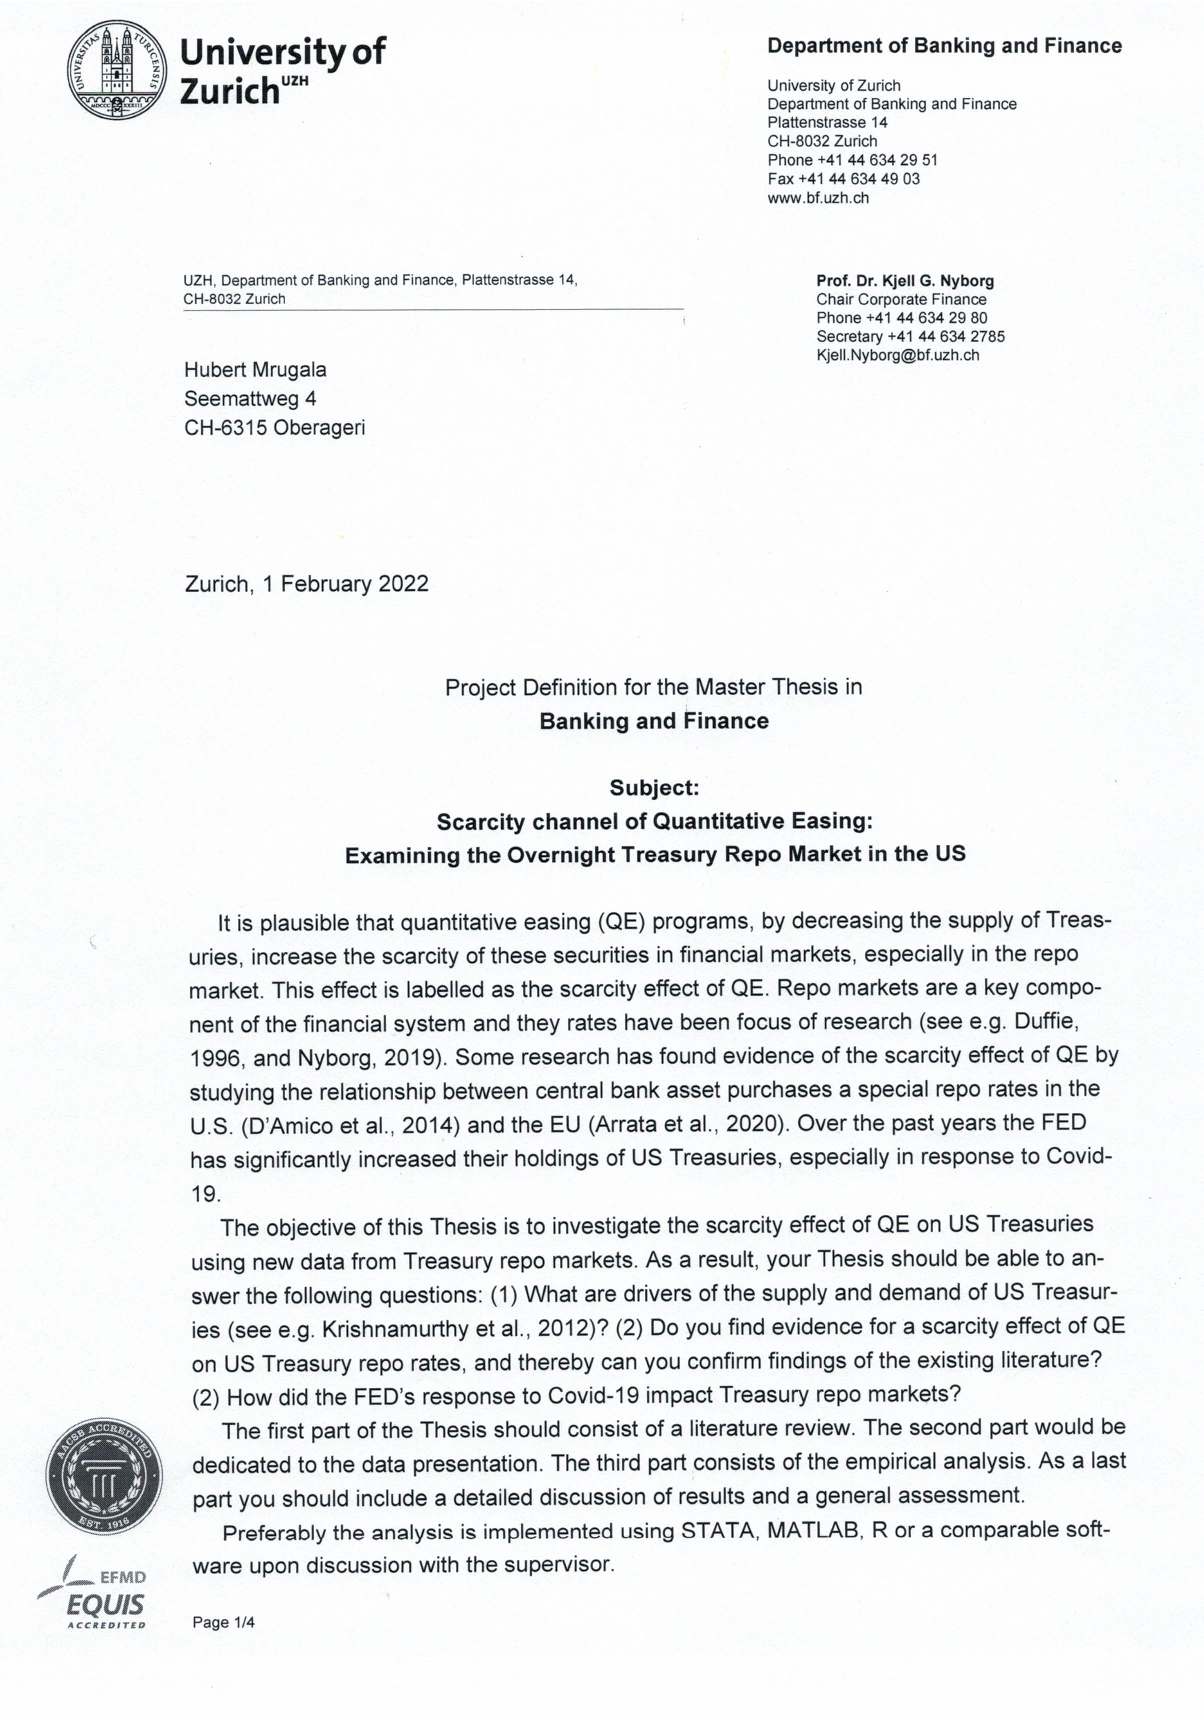
\includegraphics[page=1,width=.86\textwidth]{../../project_definition.pdf}
  \end{center}
\end{figure}
\newpage
\begin{figure}[h!]
  \begin{center}
    \includegraphics[page=2,width=.86\textwidth]{../../project_definition.pdf}
  \end{center}
\end{figure}
\newpage
\begin{figure}[h!]
  \begin{center}
    \includegraphics[page=3,width=.86\textwidth]{../../project_definition.pdf}
  \end{center}
\end{figure}
\newpage
\begin{figure}[h!]
  \begin{center}
    \includegraphics[page=4,width=.86\textwidth]{../../project_definition.pdf}
  \end{center}
\end{figure}

\thispagestyle{firststyle}
\newpage

% ----- EXEC SUMMARY AND ABSTRACT ----- 
\section*{Executive Summary}
\thispagestyle{firststyle}

\lipsum[1-3] % Here goes the text

\newpage
\tableofcontents
\newpage
\listoffigures
\newpage
\listoftables
\newpage
\pagenumbering{arabic}

\begin{center}
  {\Large \emph{\textbf{Scarcity channel of Quantitative Easing:\\
  Examining the Overnight Treasury Repo Market in the US}}}\\[4pt]
  Hubert Mrugala
\end{center}

\abstract{\lipsum[1]}

\begin{flushleft}
  \textbf{JEL classification}: E4, E5\\
  \textbf{Keyword}: Collateral, Scarcity, Treasury, Monetary Policy, Repo Market
\end{flushleft}

% ----- INTRODUCTION ----- 
\section{Introduction} \label{sec:introduction} % 3.5 - 4 pages

The COVID-19 pandemic has caused the deepest US recession since the Great Depression and induced the biggest monetary stimulus since the Global Financial Crisis. One of the monetary policy tools that was activated during the pandemic was an additional round of quantitative easing.\footnote{It was actually an acceleration of already present QE that was sparked by 2019 repo rumble.} In the time of 4 months, the Fed's balance sheet exploded from \$4.2 to \$7.1 trillion, and then kept growing. As of April 2022, total assets of the Fed reached almost \$9 trillion. Central bank asset purchases are used in normal times as a unconventional policy that helps achieving ultimate goals of the Fed, which are maximum employment and inflation level at 2\% over the longer run.

There are many theoretical transmission channels of quantitative easing, however almost all of those channels focus on positive effects of asset purchases. Negatives are very rarely analysed. \citet{nyborg2015} showed that collateral frameworks of ECB distort financial markets' efficiency by making bad collateral look better then it really is. What about a high-quality collateral? Can draining fist-class collateral out of the markets have an adverse impact on the economy?

There is one channel of quantitative easing that is rarely mentioned and insuffitiently studied.\footnote{In financial media, only Izabella Kaminska of FT Alphaville sometimes covered collateral scarcity.}. It is the scarcity channel (or scarcity effects). While most channels on QE focus on abundance of reserves, central bank liquidity, the scarcity effect, puts emphasis on the collateral-side of the swap, which is the public sector liquidity. There are only two academic papers that study the scarcity channel of asset purchases programmes. \citet{damico2014} find that there was a scarcity premium of US Treasury securities traded in the repo market during the time of LSAP programs. Likewise, \citet{arrata2018} determine a similar relationship in the \textbf{Euro zone market for repo contracts}. Both papers prove the existence of the scarcity effects in the US and EU markets, however, those investigations look only at specific special repo markets and don't take into account the mechanics of the collateral intermediation complex. Furthermore, there hasn't been any research done about the scarcity premium of US Treasuries in over eight years, despite an almost constant QE during that period.

This research fills the subject gap, the time gap, and the context gap in the narrow literature on scarcity effects. I use a General Collateral Financing Treasury Repo rate weighted index in a timespan of the last 15 years to test a connection between the level of US Treasury securities on the Fed's balance sheet and the index. Additionally, to focus completely on the collateral-side of a repo transaction, I use a collateral spread as the dependent variable. \citet{nyborg2019b} \textbf{find ...}

\textbf{[Findings]}

I control for \textbf{[...]} and emphasize the importance of high-quality collateral by describing its dynamics and economic function. Moreover, I add an innovative proxy for the re-use rate of collateral in the banking system as an extension of the base model.

The research connects three different strains of literature, which are research on collateral scarcity, US Treasury markets and collateral intermediation.

Apart from already mentioned academic papers on scarcity effects, there is also one investigation of the Japanse JGB market that contributes to the literature on collateral scarcity. \citet{han2018} have documented that BoJ purchases of Japanese Government Bonds in QE and then QQE programs have negative impact on market liquidity, which suggest scarcity effects.

The second stain is the literature on repo market rates and cash market rates of US Treasuries. The work of \citet{duffie1996} introduced a model that shows how short-selling Treasuries obtained by reverse-repo transactions can create squeezes at delivery dates and so, cause some repos to trade on special. Special repo rates are not studied in this research, however, mechanics of special repos are important because US Treasuries, as a whole asset group, are special on their own. \citet{krishnamurthy2012} show that yields of US Treasury securities have a non-default component that makes them trade at a significant premiu. 

The last branch of literature is concerned with the collateral supply and its intermediation. \citet{singh2011} shows how collateral agency is embedded into the shadow banking system. \citet{sissoko2020} show how sufficient collateral supply is crucial to properly functioning money markets and effective monetary policy. \citet{singh2012} introduce and explain a phenomenon of "collateral-chains". \citet{singh2017} calculates the collateral re-use rate that represents endogenous shadow creation of collateral. \citet{jank2021} finds a positive relationship between ECB bond purchases (PSPP) and the re-use rate of collateral suggesting that the market participants adjust to shocks in collateral scarcity by utilizing more source collateral.

Investigating scarcity effects of unconventional monetary policy is important because it is not certain that government bond purchasing programs of central banks have a net positive effect on the real economy. Benefits of QE or PSPP are not clear. Despite over 10 years of bloated central bank balance sheets, inflation and growth did not follow.\footnote{According to \citet{gern2015}, increase in GDP and inflation are two final effects of the QE/PSPP transmission mechanism.}. If scarcity effects are large and significant, then a lack of central bank unsterilized actions in response to an external shock may be more beneficial than active bond purchases. Nonetheless, the final assessment must be made by looking at the bigger picture and taking into account other factors like the regulatory environment and demand for reserves. This work studies only scarcity effects. \textbf{Last but not least, scarcity effects and connection to .. may shed a light on why some central banks decide to apply controvenial collateral frameworks.}

% Figure: Fed's BS
\begin{figure}[htb!]
  \begin{center}
    \caption{The long-term rate has been very low in spite of massive QE}
    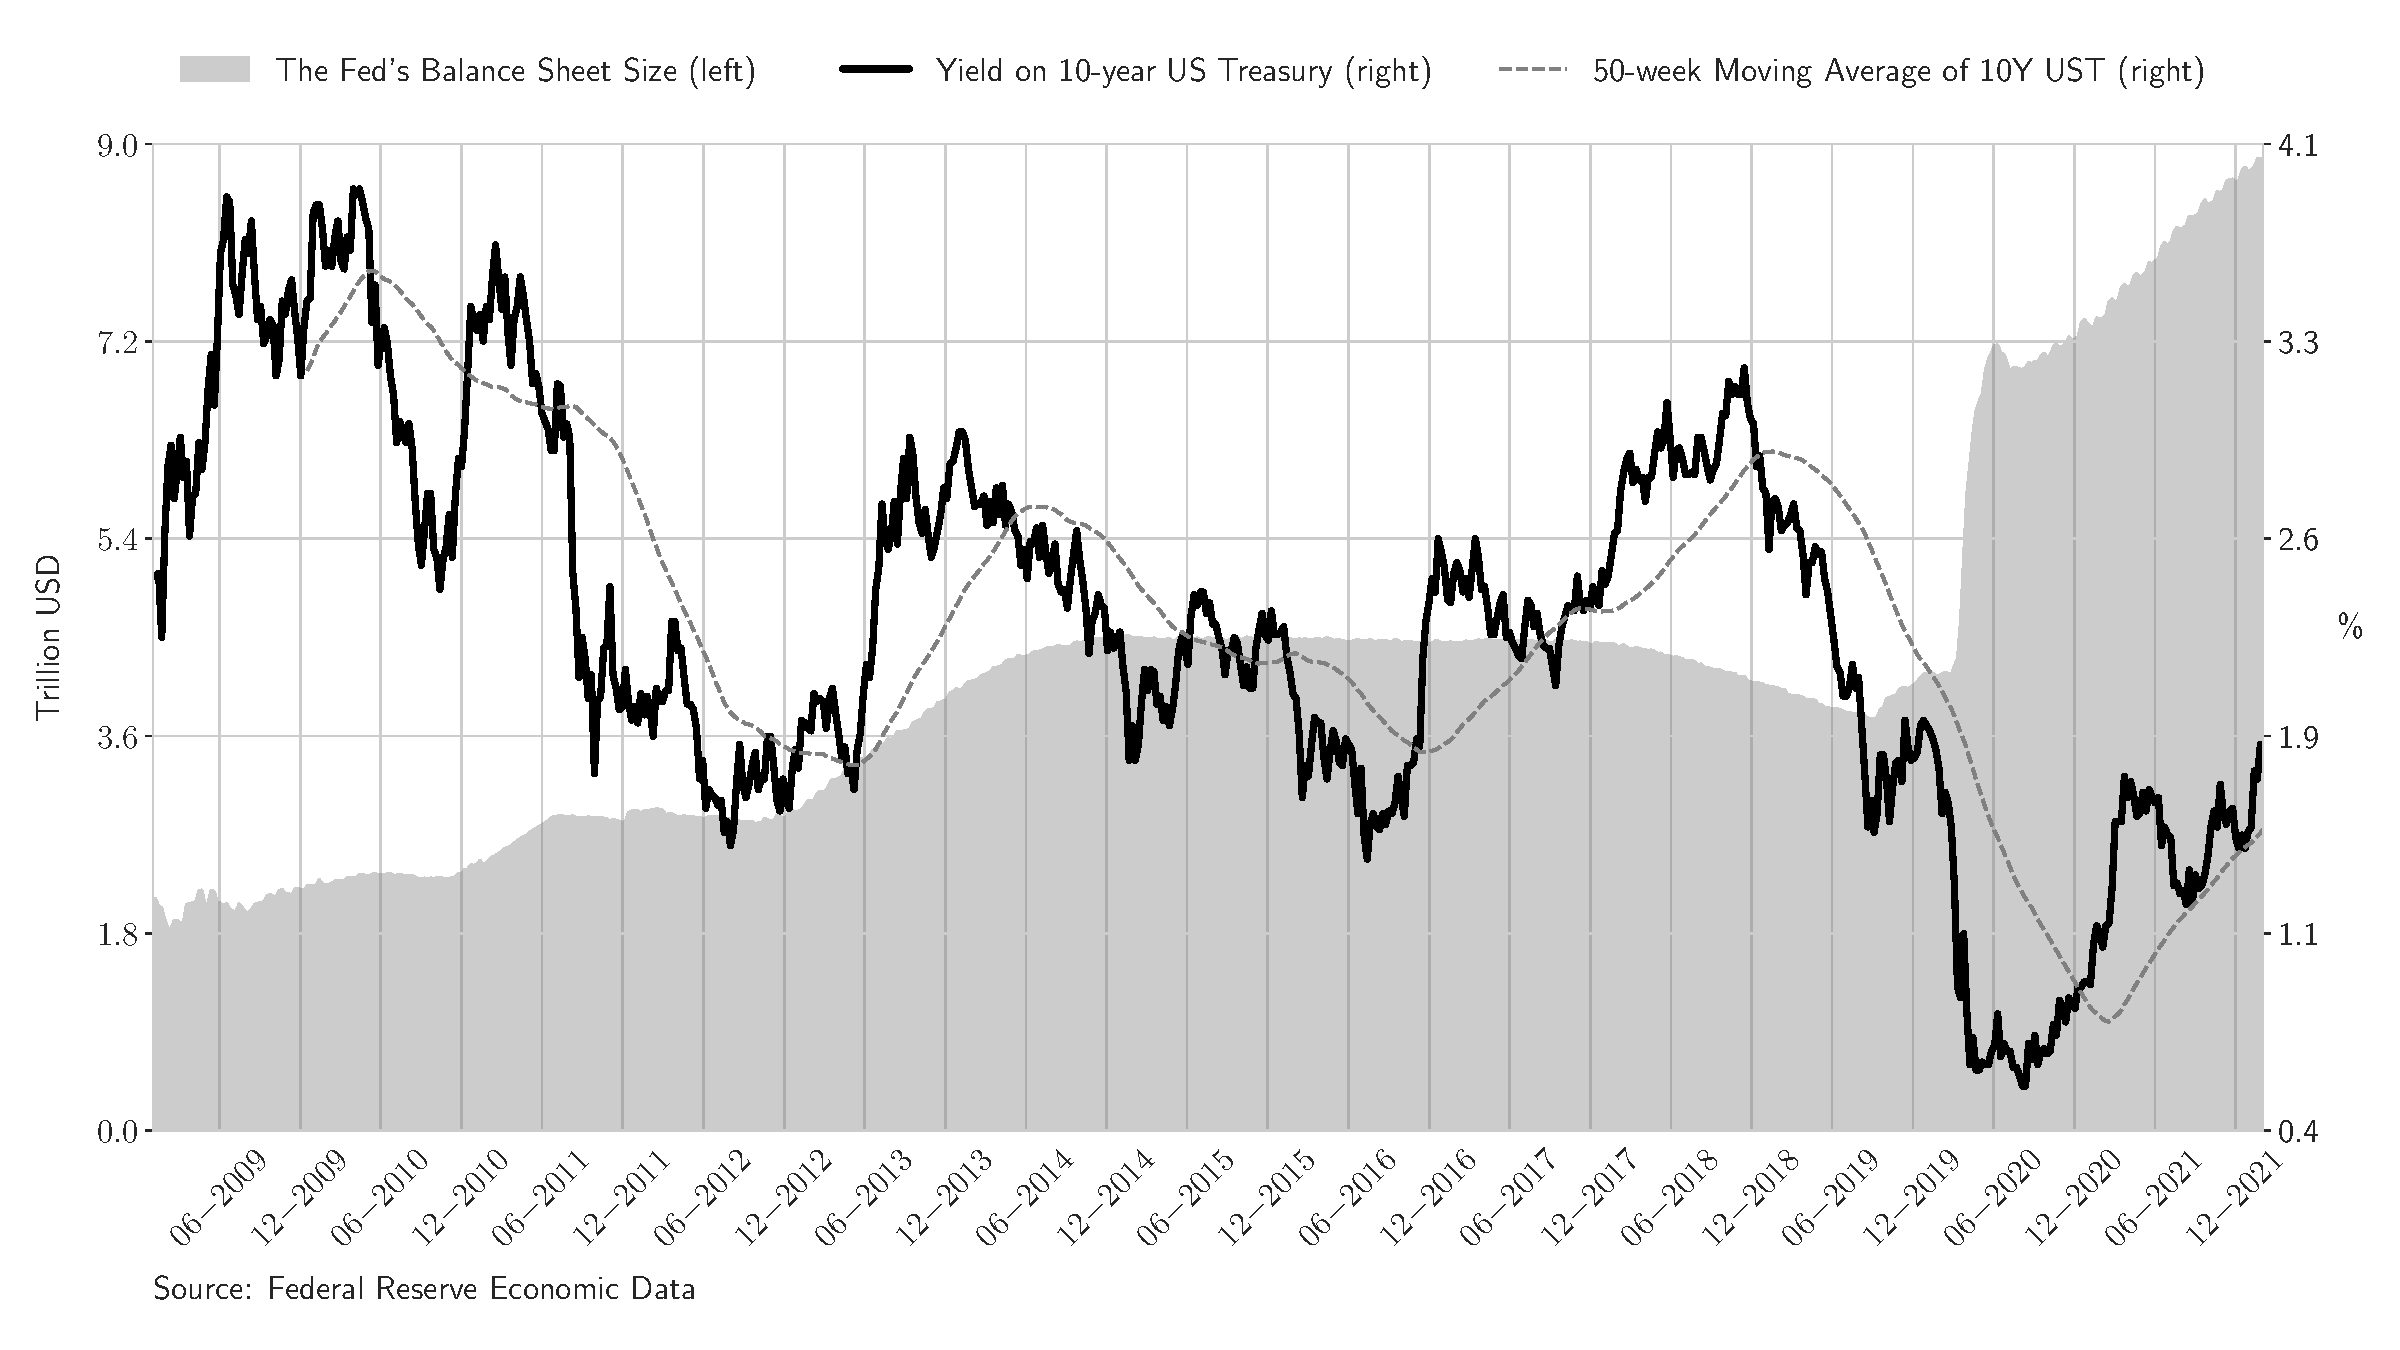
\includegraphics[width=0.99\linewidth]{fed_bs.pdf}
  \end{center}
  \label{Feds_BS}
\end{figure}

The remainder of the paper is organized as follows. \textbf{Section two. Section three.} The last section concludes.

\newpage

% ----- COLLATERAL MECHANICS ----- 
\section{Mechanics of collateral} \label{sec:mechanics} % 3-4 pages

\subsection{Collateral and the repo market} % 2 pages

\subsection{Collateral flows} % 2 pages

\subsection{Off-balance sheet collateral} % 2 pages

\newpage

% ----- COLLATERAL SHORTAGE ----- 
\section{Collateral shortage in years 2020-2022} \label{sec:shortage}% 3-4 pages 

\subsection{Treasury bill scarcity} \label{sec:bills}

\subsection{Fed's reverse repo standing facility} \label{sec:rrp}

\newpage

% ----- EMPIRICAL ----- 
\section{Empirical tests} \label{sec:empirical}

% Data
\subsection{Data} \label{sec:data}

The three main variables that are studied in this research are: the Fed's System Open Market Account (SOMA) Treasury holdings, General Collateral Finance (GCF) Treasury overnight repo rate and the USD collateral spread.

Repo rate data comes form The Depository Trust \& Clearing Corporation (DTCC). The rate is a weighted-average rate of repo contracts that are backed with repo-eligible Treasuries with maturity less than 30 years (CUSIP: 371487AE9). It tracks the average daily interest rate paid for the most-traded GCF Repo contracts for US Treasury securities. DTCC a of clearing house for trading US government securities.

Collateral spread is the difference between an unsecured and secured money market rate. An unsecured financing normally is more expensive that a secured one, since secured lending (e.g. a repo contract) is safer to the leg that lends legal tender money. That is not always the case as showed in figure \ref{fig:collateral spread}. \citet{nyborg2019a} explains what drives collateral spread and makes at times to turn negative. Here, the collateral spread, for the US market, is defined as the difference between overnight USD LIBOR rate and the overnight GCF Treasury repo rate. Expressing the repo rate in the form of a collateral spread is important when analysing dynamics of collateral and it's impact on money markets. % It is because a collateral spread expresses the premium lenders pay for security.

Scarcity effects should be most visible in the repo rate because engaging in a reverse repo contract is the cheapest way of obtaining collateral securities. This analysis uses a general collateral repo rate, as opposed to a special repo rate. The reason for such decision is twofold. First, there haven't been done any studies on scarcity effects that investigate a general collateral (GC) repo rate on a macro level. Second, data for the rate is easily accessible online. Using a GC rate is convinient because of the fact, that in regression studies, there is no need to control for specialness and short selling of a "special" security. On the other hand, it is hard to include the market microstructure factors when using a general collateral rate, especially with the weekly data frequency that is applied in this study.

To gauge the volume of Treasury securities on the Federal Reserve balance sheet, I use the System Open Market Account Holdings (SOMA) data. SOMA holding are Fed's assets acquired via open market operations. To make the data relevant for this study, I sum only Treasury bills, notes and bonds and leave out mortgage backed securities and federal agency securities.

Increase in the Fed's SOMA Treasury holdings reduce the supply of government security collateral, however, increase in the outstanding security debt has the opposite effect. I use Debt to Penny daily data of all federal debt outstanding, except debt held by intragovernmental holdings. This time-series is re-sampled to weekly Wednesday levels to match the frequency of the Fed's Treasury holdings.

The recently popular reverse repo standing facility of the Federal Reserve can alleviate any potential shortage of Treasury collateral, thus I also include these figures as well. For a more detailed analysis of the Fed's RRP sale volumes, please see section \ref{sec:shortage}.

To control for other factors that move the repo rate and collateral spread I include three other variables, namely VIX index, 1-month yield on US Treasury bill and a yield curve defined as 10-year UST yield less 3-month UST yield. All non-dummy variables are defined in table \ref{table:variables}.

Lastly, there are four categorical variables used to control for changes in the Fed's monetary policy stance. Two of them show when the Fed rises or lowers the fed funds target rates, and the other two indicate dates when the Fed expands and normalizes its balance sheet. The dates can be seen in table \ref{table:dates}, in the appendix section.

% Table: Variables
\begin{sidewaystable}[htbp!] \centering
\caption{Explanation of variables.\\
  All data was accessed and transformed on 10th March 2022.}
{\renewcommand{\arraystretch}{2.2} 
\begin{tabular}{lll}
\toprule
  \textbf{Variable} & \textbf{Definition} & \textbf{Source} \\
\midrule
  TREASURY REPO RATE &  \makecell[l]{GCF (General Collateral Finance) Treasury repo rate\\weighed index composed of GCF repo-eligible CUSIPs:\\U. S. Treasury $<$ 30-year maturity, in bps} & www.dtcc.com\\
\hline
  LIBOR & ICE "Panel Bank" Overnight USD LIBOR rate, in bps & Bloomberg\\
\hline
  COLLATERAL SPREAD & USD ON LIBOR rate minus the Treasury repo rate, in bps & \\
\hline
  UST 1M & Yield on generic 1-month US Treasury bill, in bps & home.treasury.gov\\
\hline
  YIELD CURVE & \makecell[l]{10-year US Treasury note yield  minus 3-month US Treasury\\bill yield, in bps} & home.treasury.gov\\
\hline
  SOMA TREASURIES & \makecell[l]{Fed's Treasury securities at System Open Market\\Account holdings, tril USD} & www.newyorkfed.org\\
\hline
  DEBT & Debt held by the public (debt to penny data), in tril USD & fiscaldata.treasury.gov\\
\hline
  RRP & \makecell[l]{Fed's Overnight Reverse Repurchase Agreements -- Treasury\\securities sold by the Federal Reserve in the temporary\\Open Market Operations, in tril USD} & fred.stlouisfed.org\\
\hline
  VIX & Chicago Board Options Exchange's CBOE Volatility Index & finance.yahoo.com\\
\hline
  PD FAILS & \makecell[l]{Repo fails to receive and fails to deliver, US Treasury\\securities, Primary Dealer Statistics, in tril USD} & www.newyorkfed.org \\
  \bottomrule
\end{tabular}}
% \begin{flushleft}
% \hspace{35pt}\textit{* .}
% \end{flushleft}
\label{table:variables}
\end{sidewaystable}

The time range of the whole data set\footnote{Except primary dealer statistics data that is used in one regression in the appendix.} goes from January 2, 2008 to December 29, 2021. All data has weekly frequency, Wednesday levels. Dollar values are in trillion USD, rate values are in basis points (bps). Table \ref{table:stats} shows descriptive statistics of the data used in regression analysis. All of the data, except the LIBOR rate, comes from free online resources. For detail, please see table \ref{table:variables}.

% Expand this section by adding details about those varaibles

% Stats
\subsection{Descriptive Statistics} \label{sec:stats}

Figure \ref{fig:vars} shows the evolution of the main variables in the last 11 years. The period of the two years that precede the onset of the 2020 pandemic, was the time of balance sheet normalization. Quantitative tightening started at the end of October 2017 and lasted almost two years until the repo rumble on 17th September 2019. Over that period, the Fed allowed Treasury securities and mortgage-backed securities to roll off their balance sheet. The pace of reducing Treasury holdings was \$12 billion per month, on average. At the same time the general collateral Treasury repo rate often spiked above the Fed funds upper target and the collateral spread, for almost the whole period, was negative. Interestingly, during times of QE and "taper", when securities weren't systematically bought or sold by the Fed, the collateral spread never stayed negative for so long as it did during the QT.

Table \ref{table:stats} shows basic statistics of the dataset. The average value for the collateral spread, including year 2008, was about 2.9 basis points. If we exclude the whole year 2008 from the sample, the average value changes to -1.5 basis points (median is -0.8). This implies that since 2009, the secured rate for interbank liquidity was lower than the secured one. The observation is bizzare, to say the least, since secured lending is much safer than lending that takes place without pledging any collateral.

The average pace of the US debt expansion before the 2020 pandemic was \$760 billion per month. From March 2020 to the end of 2021, the total value of the US debt increased by \$5.3 trillion, which is 30\% of March 2020 level.

The standing reverse-repo facility was opened for the first time in the data sample in September 2013. Since that date, until the end of 2017, the average volume of overnight RRP Treasury sales was about \$110 billion. The RRP facility exploded in June 2021 when the Fed added the facility again. Since May 2021, Fed's RRP overnight Treasury sales increased from about \$0.25 trillion to over \$1.6 trillion at the end of the year.

% Figure: Main variables
\begin{figure}[htb!]
  \begin{center}
    \caption{Development of primary variables.}
    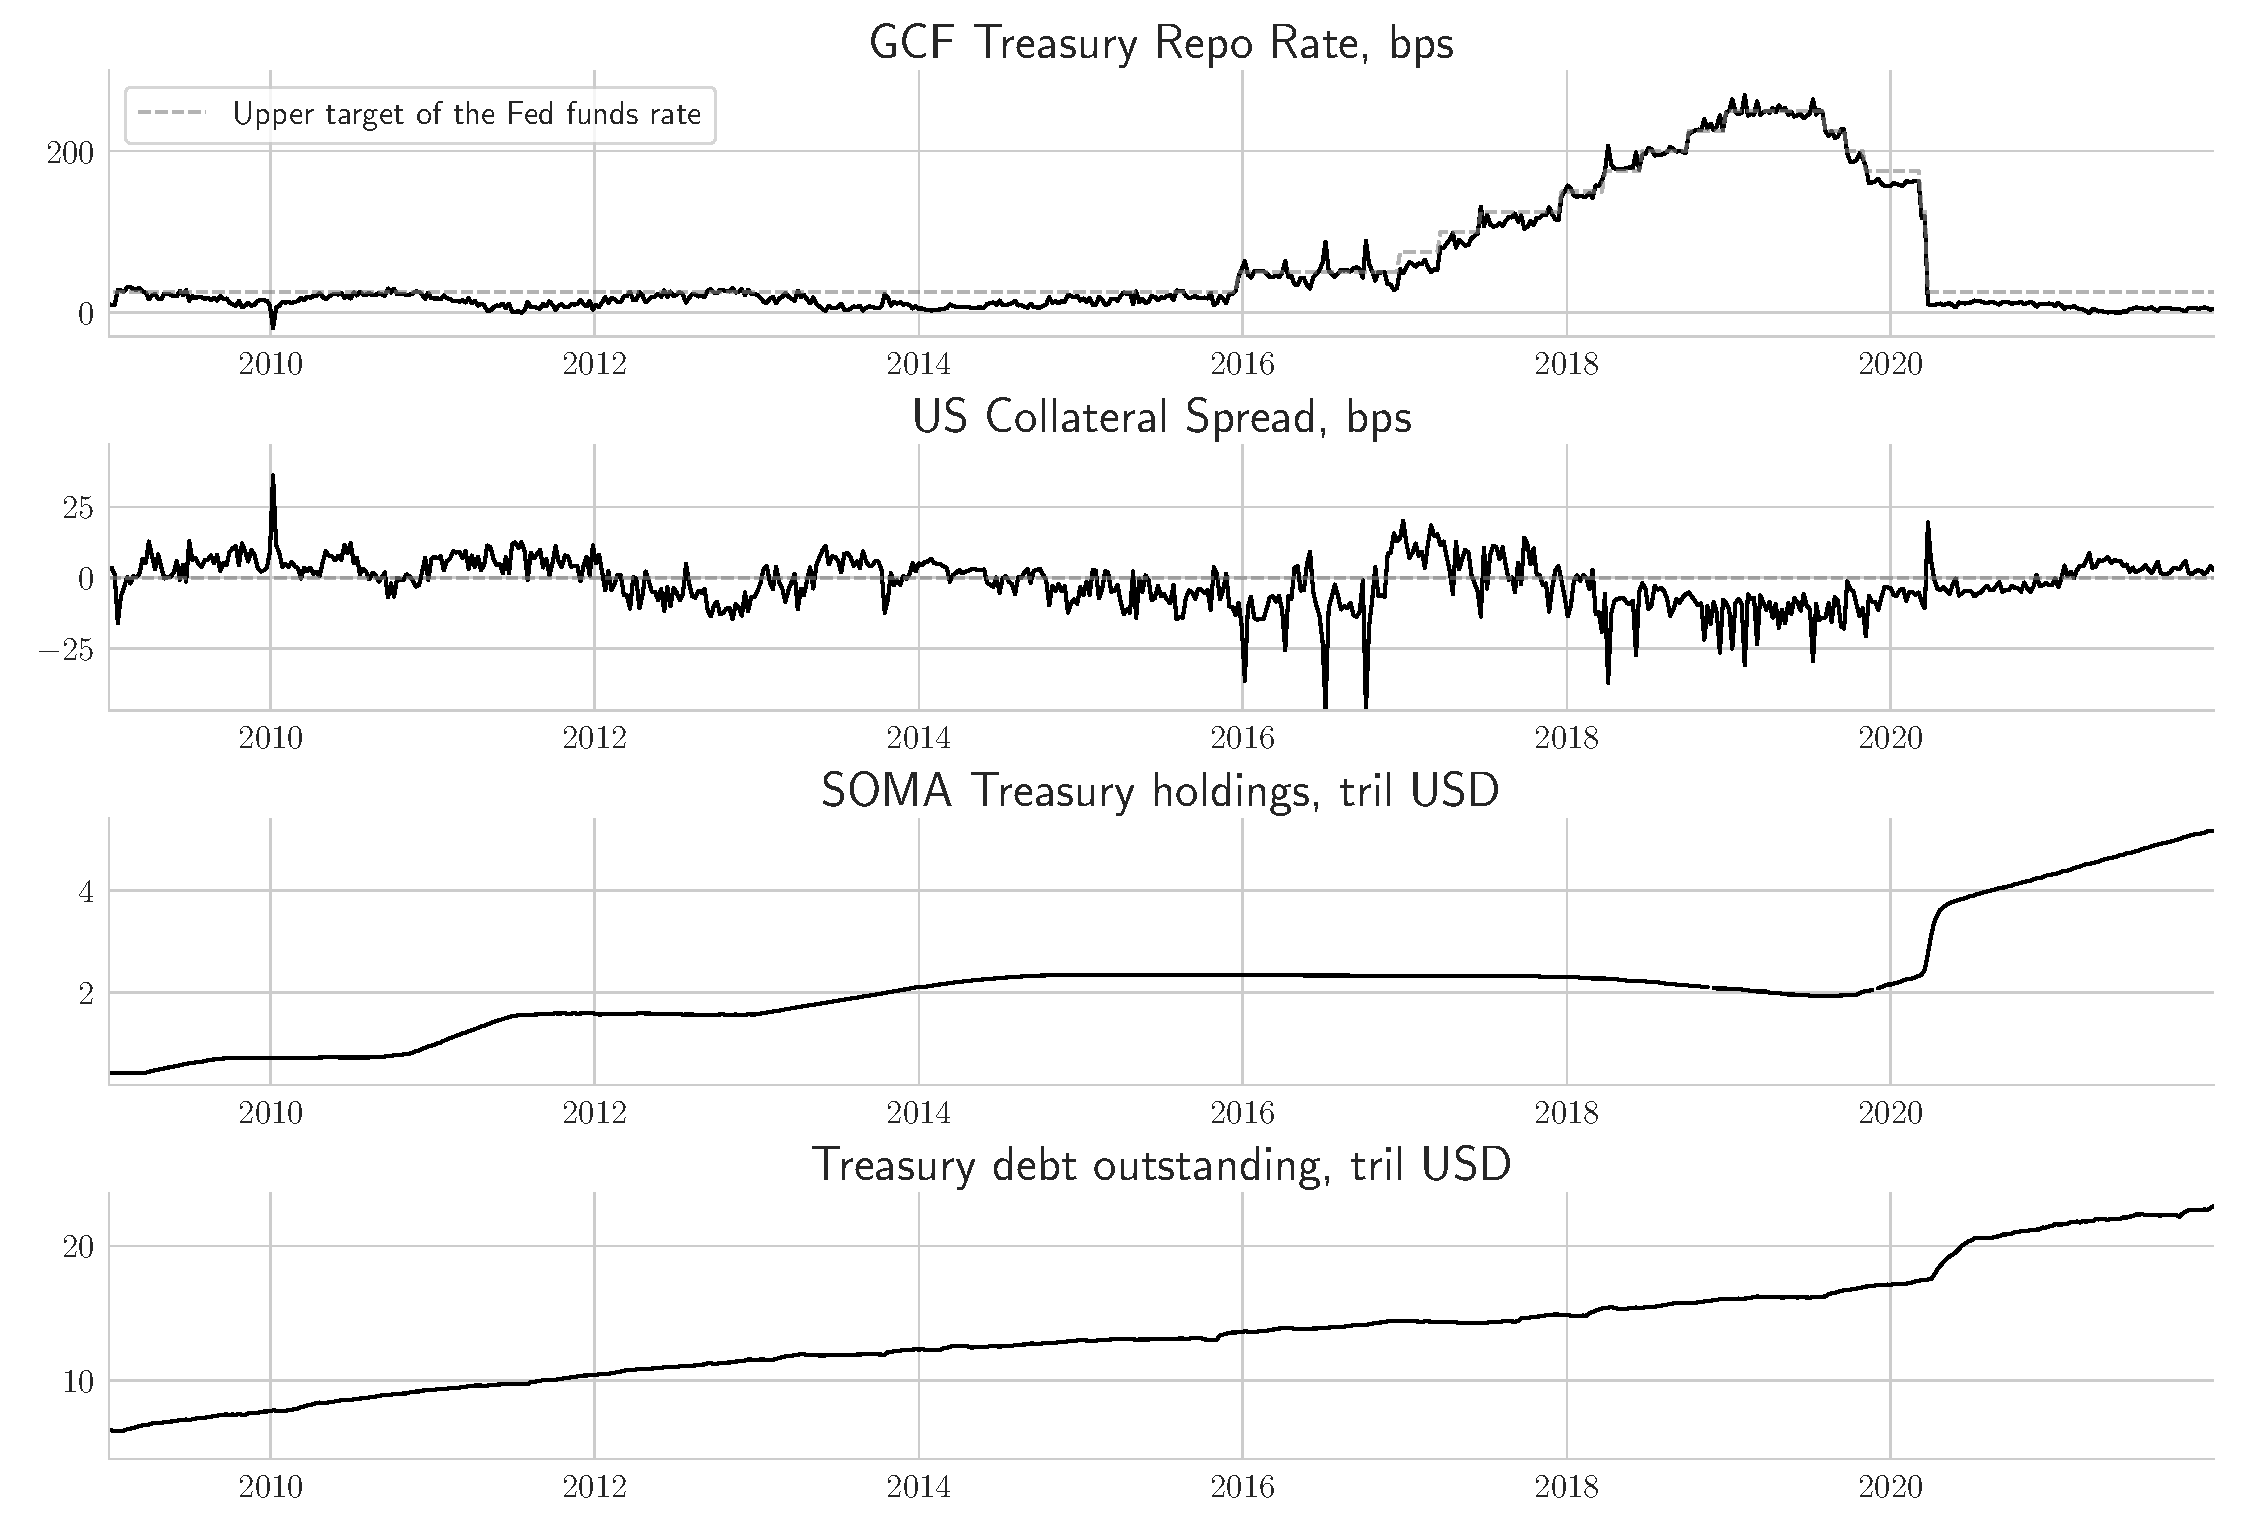
\includegraphics[width=0.99\linewidth]{main_vars.pdf}
  \end{center}
  \label{fig:vars}
\end{figure}

% Table: Statistics
\begin{table}[!h] \centering
\begin{threeparttable}
\caption{Descriptive statistics.}
\begin{tabular}{lrrrrr}
\toprule
{} &    mean &    min &     max &    std &  obs \\
\midrule
GCF Treasury O/N repo rate (bps) &   64.00 & -19.30 &  418.40 &  82.63 &  732 \\
Collateral spread, USD (bps) &    2.89 & -47.11 &  495.28 &  29.63 &  731 \\
O/N USD LIBOR rate (bps) &   66.97 &   5.46 &  509.38 &  87.47 &  731 \\
1-month UST yield (bps) &   51.52 &   0.00 &  337.00 &  77.08 &  732 \\
10-year less 3-month UST yield (bps) &  183.24 & -49.00 &  380.00 &  96.53 &  732 \\
Treasury SOMA holdings (tril USD) &    2.04 &   0.43 &    5.17 &   1.12 &  729 \\
Treasury debt outstanding (tril USD) &   13.00 &   5.10 &   23.03 &   4.47 &  732 \\
Fed's RRP standing facility volume (tril USD) &    0.09 &   0.00 &    1.70 &   0.25 &  732 \\
VIX volatility index &   20.15 &   9.19 &   80.86 &   9.76 &  732 \\
% Treasury security repo fails (all fails) &    0.19 &   0.06 &    0.89 &   0.11 &  457 \\
\bottomrule
\end{tabular}
Observations from January 2, 2008 to January 5, 2022. The data above is not transformed, however, regressions in the following section apply first-differencing.
 % (except the last variable which data starts from April 3, 2013)
\label{table:stats}
\end{threeparttable}
\end{table}

% Base model
\subsection{Base regression specification} \label{sec:base}

The main objective of this paper is to determine whether Fed's Treasury buying programs make Treasury securities more scarce in the market. To see that, I test a casual connection between Treasury security supply factors and the GCF Treasury repo rate with a simple linear regression. All data put into regressions is in first differences in order to remove trends and make time-series stationary.

There are two sets of OLS regressions with two different dependent variables. My basic regression specification involves the general collateral repo rate as the dependent variable and a set of independent variables that reflect supply and demand factors for collateral. The following is the base regression equation

\begin{equation} \label{eq:1}
  \begin{gathered}
  \Delta \textit{Treasury Repo Rate} = \beta_0 + \beta_1 \Delta \textit{SOMA Treasury}_t + \beta_2 \Delta \textit{Debt}_t \\ + \beta_3 \Delta \textit{RRP}_t  + \beta_4 \Delta \textit{UST 1M}_t + \gamma \textit{Controls}_{i,t} + \epsilon_{t}
  \end{gathered}
\end{equation}

$\Delta$ SOMA Treasury and $\Delta$ Debt variables are supply factors of the underlying collateral. The former shows to what extend the Fed draws Treasury securities out of the market and the latter variables represents provision of collateral to the market.

Fed's RRP standing facility sales are initiated by agents that seek to lend reserves to the central bank. Therefore, Treasury sales that go through the RRP facility are a demand factor for collateral. RRP volume alone cannot capture all of the demand that exist for liquid Treasury securities. It is so because only eligible parties can access central bank facilities and the price of those reverse-repo contracts is set only by the Fed. In order to account for demand for Treasury securities in the wider market, I use the $\Delta$ UST 1M variable, which is a yield on generic one month Treasury bill. \textbf{The quality of the underlying collateral affects repo rates as showed by Bartolini et al and Nyborg. Consequently, as the yield of the underlying security rises, the repo rate should also increase}.

To capture the effect of other determinants of the repo rate I incorporate three more macro variables, as well as four categorical variables that control for changes in monetary policy. Those additional macro variables are the VIX stock volatility index and the UST yield curve.

% Problem with the unsecured rate
\subsection{Problem with the unsecured rate} \label{sec:unsecured}

Repo contracts aren't all about the collateral but also serve as an instrument that provides cash liquidity to the buyer. Sometimes repo rates react more to the "collateral leg", that's when the rates plummet, but usually repo rates respond more to the "cash leg", that is driven by the demand for funds. Thus, it is essential to account for demand for cash liquidity factor, that is not associated with collateral when examining repo rates.

The unsecured rate, which in this case is the US dollar O/N LIBOR rate is an important component that indicates the price of dollar liquidity. However, it would be reckless to include it in the regression as a right-hand side variable because of a potential reverse causality problem.

Since the Global Financial Crisis, activity in the unsecured money market segment have been declining. In 2003, the split of the total lending turnover was roughly equal, but by 2015 the size of the unsecured market was only one-tenth of total \citet{fiore2018}. Much more bigger and liquid secured markets imply that a demand for funds should be first and foremost captured in repo contracts that are "cash-leg" driven. In short, it should be the secured rate that sets the price of overnight money, which then feeds into the rate of unsecured funds, and not the other way around.

The problem of a possible reverse causality may not be as big as I render it. However, the fact that the USD ICE LIBOR rates use panel bank methodology, which essentially is a daily survey, coupled with a well-known relative illiquidity and tiny size of the fed funds market, suggest that it would be wise to carefully tackle this issue.

\begin{equation} \label{eq:2}
  \begin{gathered}
    \Delta \textit{Collateral Spread} = \beta_0 + \beta_1 \Delta \textit{SOMA Treasury}_t + \beta_2 \Delta \textit{Debt}_t \\ + \beta_3 \Delta \textit{RRP}_t + \beta_4 \Delta \textit{LIBOR}_t + \beta_5 \Delta \textit{UST 1M}_t + \gamma \textit{Controls}_{i,t} + \epsilon_{t}
  \end{gathered}
\end{equation}

A simple substitution of collateral spread for the repo rate should solve this issue and make the model more robust. The collateral spread, being the difference between the unsecured and secured rate, should remove most of the variability that is caused by the demand for funds as both rates will respond to these occasions in the same direction. For this reason, the second specification sets the collateral spread as the dependent variable and puts the O/N USD LIBOR rate on the right-hand side of the equation to control for any tightness in the unsecured market. Conditions in the unsecured interbank market for liquidity still affects the collateral spread \citet{nyborg2019a}, so the unsecured rate is still included as the depended variable, but the reverse causality problem is avoided.

Other known determinants or the collateral spread are liquidity and volatility of the underlying security, haircut and risk-aversion. Regarding attributes of the underlying security in the cash market, it is not clear which security in particular should be analyzed as my repo rate cover a wide variety of Treasuries. For instance, on-the-run Treasury bills are much more liquid than off-the-run Treasury bonds. Thus, I don't use any liquidity metric and for I proxy the overall volatility in the markets as well as risk-aversion with the VIX index. Haircuts are not taken into account as all Treasury securities are deemed to have the same level of safety.

There is also one Treasuries supply factor that should be included in my regressions but isn't due to the unavailability of a high-frequency metric for that factor. It is a variable that represents the rehypothecation of collateral in the monetary system. The more often collateral is re-used collateral in the system, the higher the overall supply of collateral. Some banks put the amount of received  collateral that is allowed to be repledged in their quarterly reports. Unfortunately, the size of that data is too small to be meaningful given the time frame of this study.

% Results
\subsection{Results} \label{sec:results}

The two sets of regressions, which results are shown in the tables below confirm the hypothesis that the Fed's purchases of Treasuries put a downward pressure on the GCF Treasury repo rate, and so a upward pressure on the US collateral spread. A high and statically significant coefficient for the SOMA Treasury holdings variable in each regression specification suggest that the scarcity effects from quantitative easing programs are real.

Table \ref{table:reg1} shows how supply factors of US Treasury collateral affect the general collateral Treasury repo rate. The coefficient next to "SOMA TREASURY" variable in the second column of the table (-45.55) implies that a \$1 trillion Treasury purchase by the Fed causes the repo rate to decline, on average, by 45 basis points, with all other determinants held constant. The magnitude of the effect is much smaller than in \citet{damico2014}, however, that study is much different as it looks on special repo rates as opposed to the general collateral repo rate.

Four regressions are included in table \ref{table:reg1}, where the dependent variable is the GCF Treasury repo rate. The fist column looks only at the value of US Treasuries on the Fed's balance sheet and the total value of US Treasury debt outstanding. \citet{damico2014} and \citet{arrata2018} merge two of these values into one variable, that is a ratio of the former to the latter. Here, I put those variables separately to understand a relative magnitude of both. As illustrated in the table, taking high-quality collateral out of the market affects the repo rate more than the US Department of Treasury provision of these collateral securities. The second column adds other important factors that move the repo rate. All of them are statistically significant. Including those factors addresses the omitted variable bias, as both coefficients of SOMA and debt variables are much smaller after the addition of new variables in the model.

Columns 3, adds the overnight US dollar LIBOR rate. It doesn't change much as the coefficient of the LIBOR rate is small. Moreover, there are possible reverse causality problems when adding this variable, and its statistical explanatory power is very low. The problem with the unsecured rate in this regression setting is explained in section \ref{sec:unsecured}.

I exclude a possibility of reverse causality of the dependent variable and the main regressor, which is the Fed's Treasury holdings. The reason for this is the fact that the Fed had tried to alleviate the scarcity effect of bond purchases only once. It was done thorough a regulatory instrument, by granting a Supplementary Leverage Ratio (SLR) relief to banks in March 2020. A temporary exclusion of Treasuries and central bank reserves definitely freed up some balance sheet space of banks and allowed those banks but it had nothing to do with Treasury purchases under QE programs. Moreover, the SLR relief probably targeted the increasing size of reserves in the banking system more than the functioning of Treasury markets.

The last column adds the VIX index and  dummy variables that represent the dates when the Fed clearly took action in regard to the size of their balance sheet. Initiating or expanding quantitative easing contributed to rising repo rate, and doing the opposite, seemingly, decreased the dependent variable. However, the coefficient of the last variable, which is a dummy for tightening balance sheet dates, is not statistically significant. The coefficient of the implied volatility index is also not significant.

There are two reasons why adding those QT dates to the regression generates more noise in the model. First, quantitative tightening is a very careful and gradual process. This is contrary to announcements of QE programs, which are often sudden and act as a response to an economic or monetary crisis. Second, dates of the termination of some liquidity providing programs sometimes overlap with extension or start of other asset purchasing programs. For instance, on June 2020 the Fed stopped supporting the repo market, which was an effect of the stress in that market that started on 17th September 2019, but was still buying securities on a massive scale under the QE4 program. These quantitative easing/tightening dates can be found in table \ref{table:fed} in the appendix.

% Regression table 1: GCF repo rate
\begin{table}[!htbp] \centering
\caption{Regression --- GCF Treasury repo rate and the supply of Treasury securities}
\begin{tabular}{@{\extracolsep{5pt}}lcccc}
\\[-1.8ex]\hline
\hline \\[-1.8ex]
& \multicolumn{4}{c}{\textit{Dependent variable: GCF Treasury repo rate}} \
\cr \cline{4-5}
\\[-1.8ex] & (1) & (2) & (3) & (4) \\
\hline \\[-1.8ex]
 Intercept & -0.818$^{}$ & -0.265$^{}$ & -0.256$^{}$ & -0.366$^{}$ \\
  & (0.568) & (0.295) & (0.293) & (0.280) \\
 SOMA TREASURY & -91.651$^{**}$ & -45.549$^{***}$ & -41.788$^{**}$ & -40.532$^{**}$ \\
  & (45.276) & (17.261) & (17.358) & (17.597) \\
 DEBT & 33.710$^{***}$ & 23.180$^{**}$ & 23.801$^{**}$ & 24.281$^{**}$ \\
  & (12.068) & (10.366) & (10.121) & (10.318) \\
 RRP & & 30.961$^{**}$ & 30.904$^{**}$ & 31.183$^{**}$ \\
  & & (13.603) & (13.664) & (13.846) \\
 UST 1M & & 0.630$^{***}$ & 0.627$^{***}$ & 0.644$^{***}$ \\
  & & (0.123) & (0.118) & (0.118) \\
 YIELD CURVE & & -0.127$^{**}$ & -0.133$^{**}$ & -0.119$^{*}$ \\
  & & (0.063) & (0.059) & (0.065) \\
 C(RATE DOWN) & & -36.442$^{***}$ & -35.779$^{***}$ & -36.258$^{***}$ \\
  & & (7.825) & (7.706) & (7.825) \\
 C(RATE UP) & & 19.735$^{***}$ & 18.211$^{***}$ & 18.103$^{***}$ \\
  & & (1.758) & (2.000) & (2.045) \\
 LIBOR & & & 0.065$^{}$ & 0.062$^{}$ \\
  & & & (0.044) & (0.043) \\
 VIX & & & & 0.105$^{}$ \\
  & & & & (0.147) \\
 C(FED EASENING) & & & & 7.963$^{**}$ \\
  & & & & (3.343) \\
 C(FED TIGHTENING) & & & & -1.934$^{}$ \\
  & & & & (1.362) \\
\hline \\[-1.8ex]
 Observations & 726 & 726 & 726 & 726 \\
 Adjusted $R^2$ & 0.020 & 0.504 & 0.509 & 0.512 \\
\hline
\hline \\[-1.8ex]
\textit{Note:} & \multicolumn{4}{r}{$^{*}$p$<$0.1; $^{**}$p$<$0.05; $^{***}$p$<$0.01} \\
\end{tabular}
\begin{flushleft}
  \textit{Notes: All variables, except categorical "C" ones, are in first-difference form. Standard errors are heteroscedasticity and autocorrelation robust (HAC) using 5 lags and without small sample correction (in parentheses). All variables are defined in table \ref{table:variables}.}
\end{flushleft}
\label{table:reg1}
\end{table}

Surprisingly, the reverse-repo standing facility had a large impact on the direction of the repo rate. It was expected to have some impact, but the magnitude of its effect is astonishing. A positive coefficient suggest that as more Treasuries are borrowed from the Fed (through a reverse repo contract), more useful collateral can be utilized by money market participants. This, in turn makes the desired collateral more plentiful, which pushes the repo rate up.

Table \ref{table:reg2} presents the results of running the second model specification. It does not differ from the former one in a great extend. The only major difference is the dependent variable, which in this case in the US collateral spread. As described in section \ref{sec:unsecured}, this transformation of the dependent variable is a simple trick that allows to include the unsecured rate in the model.

The interpretation of results in table \ref{table:reg2} is the opposite to those that are in the table \ref{table:reg1}. For example, the coefficient the variable that represents the size of SOMA holdings in the column two, which is 41.788, suggest that a \$1 trillion increase in Treasuries value at the Fed cause the collateral spread to widen by about 42 basis points. Considering, that the model controls for the LIBOR rate, we can say that the this effect is caused solely by an increasing repo rate. As the collateral spreads widens and the unsecured rate stays constant, the repo rate decreases. Hence, an opposite interpretation.

Analyzing the scarcity effects in relative terms of a collateral spread, and at the same time controlling for the price of liquidity in the unsecured market, allows to isolate and analyze the collateral-side of a repo contract. This method extracts the portion of a change in a repo rate that is associated only with the market conditions of the underlying security. The results are, however, roughly the same for both of regressions.

There are a few other repo and collateral spread drives that are not included in this study. For example, haircut of the underlying security is not included because of the class of these assets (highest-quality) and the unavailability of the data. A liquidity metric of an underlying collateral is also not included because there is no metric that aggregates and provides information about the liquidity status of all securities\footnote{For instance, on-the run Treasuries are more liquid than off-the-run Treasuries. The same goes for securities with different maturities. T-bills are more liquid than T-bonds.}. I have tried out adding other regressors (that controled for liquidity, volatility, regulatory changes) and were plausible to considerably affect the final results, but none of those variables came out to be significant (see table \ref{table:reg3} in the appendix).


Since September 2019 to the end of 2021, the Fed has purchased over \$2.5 trillion of Treasury securities from the secondary market. According to the results from table \ref{table:reg1} (column 2), this expansion of the central bank's balance sheet is associated with about 113 bps decrease in the repo rate over the whole period. At the same time the US Treasury Department, through its fiscal stimulus programs, was supplying Treasury securities to the market. Taking two effects into account, the supply factors contributed to about a 56 basis point decrease of the repo rate. There are also demand factors and other drivers of the GC Treasury repo rate that were included in this study. Nonetheless, I refrain from delving too much into interpretation of control variables as effect sizes of those additional variables very rarely have a casual interpretation \citet{hunermund2020}.

% Second column of both regression sets 

% effect of both debt and soma and rrp

% effects of policy normalization 

All regressions use Newey–West standard errors. The number of lags is equal to the closes integer of the fourth root of the number of observations (726), which is 5. Each variable, except categorical variables, is in the fist-difference form ($X_t-X_{t-1}$).

% Regression table 2: Collateral spread
\begin{table}[!htbp] \centering
\caption{Regrression --- Measuring scarcity effects with collateral spread}
\begin{tabular}{@{\extracolsep{5pt}}lccc}
\\[-1.8ex]\hline
\hline \\[-1.8ex]
& \multicolumn{3}{c}{\textit{Dependent variable: US Collateral spread}} \
\cr \cline{3-4}
\\[-1.8ex] & (1) & (2) & (3) \\
\hline \\[-1.8ex]
 Intercept & 0.933$^{}$ & 0.256$^{}$ & 0.366$^{}$ \\
 SOMA TREASURY & 25.869$^{}$ & 41.788$^{**}$ & 40.532$^{**}$ \\
  & (22.988) & (17.358) & (17.597) \\
 DEBT & -46.641$^{**}$ & -23.801$^{**}$ & -24.281$^{**}$ \\
  & (19.162) & (10.121) & (10.318) \\
  & (0.636) & (0.293) & (0.280) \\
 RRP & & -30.904$^{**}$ & -31.183$^{**}$ \\
  & & (13.664) & (13.846) \\
 UST 1M & & -0.627$^{***}$ & -0.644$^{***}$ \\
  & & (0.118) & (0.118) \\
 LIBOR & & 0.935$^{***}$ & 0.938$^{***}$ \\
  & & (0.044) & (0.043) \\
 YIELD CURVE & & 0.133$^{**}$ & 0.119$^{*}$ \\
  & & (0.059) & (0.065) \\
 C(RATE DOWN) & & 35.779$^{***}$ & 36.258$^{***}$ \\
  & & (7.706) & (7.825) \\
 C(RATE UP) & & -18.211$^{***}$ & -18.103$^{***}$ \\
  & & (2.000) & (2.045) \\
 VIX & & & -0.105$^{}$ \\
  & & & (0.147) \\
 C(FED EASENING) & & & -7.963$^{**}$ \\
  & & & (3.343) \\
 C(FED TIGHTENING) & & & 1.934$^{}$ \\
  & & & (1.362) \\
\hline \\[-1.8ex]
 Observations & 726 & 726 & 726 \\
 Adjusted $R^2$ & 0.007 & 0.770 & 0.772 \\
\hline
\hline \\[-1.8ex]
\textit{Note:} & \multicolumn{3}{r}{$^{*}$p$<$0.1; $^{**}$p$<$0.05; $^{***}$p$<$0.01} \\
\end{tabular}
\begin{flushleft}
\vspace{-5pt}
  \textit{Notes: Collateral spread is defined as the difference between USD ON LIBOR rate and ON GCF Treasury repo rate. All variables, except categorical "C" ones, are in first-difference form. Standard errors are heteroscedasticity and autocorrelation robust (HAC) using 5 lags and without small sample correction (in parentheses). All variables are defined in table \ref{table:variables}.}
\end{flushleft}
\label{table:reg:2}
\end{table}

\newpage %

% ----- CONCLUSIONS ----- 
\section{Conclusions} \label{sec:conclusion} 

% \lipsum[1-8]

% ----- APPENDIX (OPTIONAL) ----- 
\newpage

% \appendix
% \noappendicestocpagenum
%\addappheadtotoc
%\appendixpage

% \begin{appendix}
%   \section{A}
% \end{appendix}

\begin{appendices}
% \section{Tables}

% Table: Fed Dates
\begin{table}[!h] \centering
\begin{threeparttable}
\caption{Fed Dates.}
\begin{tabular}{lll}
\toprule
Date & Variable & Event \\
\midrule
25 Nov 2008 & FED EASING & Announcement of QE1 \\
16 Mar 2009 & FED EASING & QE1 Expanded \\
31 Mar 2010 & FED TIGHTENING & QE1 Terminated \\
10 Aug 2010 & FED EASING & QE1 Rollover \\
3 Nov 2010 & FED EASING & Announcement of QE2 \\
21 Sep 2011 & FED EASING & Announcement of Operation Twist \\
20 Jun 2012 & FED EASING & Operation Twist Extended \\
13 Sep 2012 & FED EASING & Announcement and initiation of QE3 \\
12 Dec 2012 & FED EASING & QE3 Expanded \\
31 Dec 2012 & FED TIGHTENING & Operation Twist Terminated \\
18 Dec 2013 & FED TIGHTENING & Start of the QE3 taper \\
29 Oct 2014 & FED TIGHTENING & QE3 Terminated \\
1 Nov 2017 & FED TIGHTENING & QT has begun \\
20 Mar 2019 & FED EASING & The Fed slows down the reduction of its Treasury holdings \\
18 Sep 2019 & FED EASING & Overnight lending repo facility opened \\
15 Mar 2020 & FED EASING & Announcement of QE4 \\
11 Jun 2020 & FED TIGHTENING & The Fed tightness operations in the repo market \\
\bottomrule
\end{tabular}
Observations from January 2, 2008 to January 5, 2022 (except the last variable which data starts from April 3, 2013). The data above is not transformed, however, regressions in the following section apply first-differencing.
\label{table:fed}
\end{threeparttable}
\end{table}

% Regression table 3: Collateral spread, additional variables NEW
\begin{table}[!htbp] \centering
\caption{Regression -- Adding other plausible explanatory variables to the collateral spread specification.}
\vspace{-10pt}
\begin{flushleft}
Variable "UST 3M BID-ASK" is the bid-ask spread of a generic 3-month Treasury bill yield. Variable "UST 3M 10W VOL" is the 10-week realized volatility of a generic 3-month Treasury bill yield. The first column regression uses a smaller data sample that starts April 3, 2013. All newly added variables are not statistically significant (p-values exceed as much as 0.3). Condition number of the third column regression is large which indicates strong multicollinearity.
\end{flushleft}
\begin{tabular}{@{\extracolsep{5pt}}lccc}
\\[-1.8ex]\hline
\hline \\[-1.8ex]
& \multicolumn{3}{c}{\textit{Dependent variable: US Collateral Spread}} \
\cr \cline{3-4}
\\[-1.8ex] & (1) & (2) & (3) \\
\hline \\[-1.8ex]
 Intercept & 0.411$^{*}$ & 0.358$^{}$ & 0.253$^{}$ \\
  & (0.237) & (0.284) & (0.294) \\
 SOMA TREASURY & 28.773$^{}$ & 21.443$^{}$ & 41.205$^{**}$ \\
  & (20.417) & (28.856) & (17.177) \\
 DEBT & -21.732$^{***}$ & -19.209$^{**}$ & -23.466$^{**}$ \\
  & (6.063) & (9.457) & (10.184) \\
 RRP & -27.035$^{**}$ & -30.481$^{**}$ & -31.166$^{**}$ \\
  & (13.337) & (13.516) & (13.612) \\
 UST 1M & 0.013$^{}$ & -0.581$^{***}$ & -0.626$^{***}$ \\
  & (0.117) & (0.154) & (0.119) \\
 LIBOR & 0.109$^{}$ & 0.951$^{***}$ & 0.937$^{***}$ \\
  & (0.276) & (0.035) & (0.043) \\
 YIELD CURVE & 0.178$^{***}$ & 0.153$^{***}$ & 0.133$^{**}$ \\
  & (0.048) & (0.055) & (0.059) \\
 C(RATE DOWN) & 6.631$^{}$ & 36.885$^{***}$ & 35.694$^{***}$ \\
  & (9.963) & (8.863) & (7.720) \\
 C(RATE UP) & -2.429$^{}$ & -19.216$^{***}$ & -18.174$^{***}$ \\
  & (6.177) & (1.903) & (1.983) \\
 PD FAILS & -0.791$^{}$ & & \\
  & (2.826) & & \\
 UST3M 10W VOL & & 0.480$^{}$ & \\
  & & (0.490) & \\
 UST3M BIDASK & & & 0.004$^{}$ \\
  & & & (0.006) \\
\hline \\[-1.8ex]
 Observations & 452 & 716 & 726 \\
 Adjusted $R^2$ & 0.096 & 0.800 & 0.770 \\
\hline
\hline \\[-1.8ex]
 & \multicolumn{3}{r}{$^{*}$p$<$0.1; $^{**}$p$<$0.05; $^{***}$p$<$0.01} \\
\end{tabular}
\begin{flushleft}
\vspace{-5pt}
  \textit{Notes: Collateral spread is defined as the difference between USD ON LIBOR rate and ON GCF Treasury repo rate. All variables, except categorical "C" ones, are in first-difference form. Standard errors are heteroscedasticity and autocorrelation robust (HAC) using 5 lags and without small sample correction (in parentheses). All other variables are defined in table \ref{table:variables}.}
\end{flushleft}
\label{table:reg3}
\end{table}

\end{appendices}

% ----- BIBLIOGRAPHY ----- 
\newpage
\bibliography{refs}

% ----- STATEMENT ----- 
\newpage
\thispagestyle{firststyle}
\section*{Eidesstattliche Erklärung}
Der Verfasser erklärt an Eides statt, dass er die vorliegende Arbeit selbständig, ohne fremde Hilfe und ohne Benutzung anderer als die angegebenen Hilfsmittel angefertigt hat. Die aus fremden Quellen (einschliesslich elektronischer Quellen) direkt oder indirekt übernommenen Gedanken sind ausnahmslos als solche kenntlich gemacht. Die Arbeit ist in gleicher oder ähnlicher Form oder auszugsweise im Rahmen einer anderen Prüfung noch nicht vorgelegt worden.\\[2cm]

\hspace{60pt} 18.05.2022

\dotbox{Ort, Datum} \hfill \dotbox{Unterschrift des/der Verfassers/in}
\end{document}
